\section{Attack overview}
\label{sec:attack}
We begin by summarizing our attack.  Our attack is based on traffic correlation,
so it requires an attacker to observe traffic that is both entering and exiting
the Tor network.  In contrast to earlier work, we consider DNS instead of just
end-to-end TCP packets.

Our attack is illustrated in Figure~\ref{fig:attack-scenario} and requires the
following building blocks:
\fixme{Figure is great, but text below needs to be reworked to fit structure
of section.}
\begin{figure}[t]
	\centering
	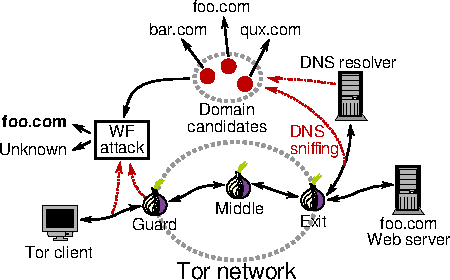
\includegraphics[width=\linewidth]{figures/attack-scenario.pdf}
	\caption{An overview of our correlation attack.  Ingress traffic is
	monitored either by a network-level adversary or the guard relay.  Egress
	traffic is monitored either by a network-level adversary or a DNS server.
	Captured DNS queries then serve as the candidate set for a Website
	fingerprinting attack.}
	\label{fig:attack-scenario}
\end{figure}

\begin{description}
	\item[Ingress sniffing] An attacker must observe traffic that is entering
		the Tor network.  The attacker can operate on the network level, i.e.,
		be a malicious ISP, or an intelligence agency.  In addition, the
		attacker can operate on the relay level, i.e., run a malicious Tor guard
		relay.  Note that in both cases, the attacker can only observe encrypted
		data.  Therefore, packet meta information such as packet lengths and
		directions serve as input to a website fingerprinting
		attack~\cite{Panchenko2016a}.
	\item[Egress sniffing] To observe both ends of the communication, an
		attacker must also observe egress DNS traffic.  We expect the adversary
		to operate on the network level, i.e., be on the path between exit relay
		and a DNS server.  Alternatively, the attacker can run a malicious DNS
		resolver or server.  Note that an attacker may also run an exit relay,
		but in that case she might as well do classical end-to-end correlation.
	\item[WF fingerprinting] We employ a website fingerprinting attack to
		determine if any of the recently observed DNS queries in egress traffic
		could be part of the encrypted ingress traffic.  Note that the DNS query
		itself does not tell us what \emph{page} a user is going to.
\end{description}

\subsection{Simulating Tor-exits' DNS traffic}
% the angle is: we have to simulate all DNS traffic from all Tor exits,
% the goal is to convince that we'ev made reasonable assumptions
To estimate the capability of an attacker, we need to investigate what
DNS data is observable for the attacker, that is what DNS request are
emerging from Tor exit relays.

We cannot use real data because there are no logs of outgoing traffic
from Tor exit relays available to us and ethical considerations kept us
from trying to collect them (\eg by operating exit relays and recording
the outgoing traffic). We therefore \emph{simulate} the DNS traffic
emerging from Tor exit relays.

\subsubsection{Website Popularity Distribution}
% powerlaw, not uniform
First, we model \emph{what websites} are visited by Tor users.
Currently, there are about 170 million active
websites\footnote{\url{http://news.netcraft.com/archives/2016/06/22/june-2016-web-server-survey.html}}
in the world and the Alexa ranking gives insights into their popularity
based on the browsing behaviour of a sample of all internet users
\footnote{\url{https://support.alexa.com/hc/en-us/articles/200449744}}.
It has been shown that the popularity of a website follows a powerlaw
distribution based on the rank of the website\fixme{citation needed}. So
we fit a powerlaw distribution to the page view numbers of the Alexa top
10\,000 websites\footnote{We used the python powerlaw package
		\url{https://github.com/jeffalstott/powerlaw} for fitting, the
		resulting powerlaw distribution had an $\alpha$ parameter of
		$1.10291152854$. Page view numbers as collected by Alexa ignore
		multiple visits by the same user on the same day, so the ranking
		might be slightly off for our purposes.} and use the result to
model which websites are visited by Tor users.
This might overestimate the popularity of higher-ranked websites because
Tor users might be visiting less popular websites, such as websites that
are censored in different parts of the world, more often than the
average internet users and we will discuss the implications of this for
our results later on.

\subsubsection{Page load frequency}
% phw's numbers extrapolated
Second, we determine \emph{how many websites} are visited by Tor users in a
certain time span. We use (less intrusive) statistics on the number of
outgoing DNS requests collected on a Tor exit relay under our control
and interpolate these numbers to all Tor exit relays based on the
published bandwidth statistics of all Tor exit relays\footnote{We found
		our exit relay \texttt{746BE73579F274AFEFA5E12C4ADACD53784D0762}
		to have on average 119.3 outgoing DNS requests per 5 minutes
		during a two week period, which corresponds to about 1.583 page
		visits per minute (taking caching into account and assuming a
		powerlaw distribution of site popularity as described above).
		The exit was configured to only allow port 80 and 443 during the
		time of the measurements to avoid counting DNS requests from
		other protocols than HTTP and HTTPS. We then used the
		self-reported bandwidth information from Tor exit relays
		collected in the ``extra-info'' descriptors available on
		\url{https://collector.torproject.org/} to estimate the number
		of page loads on each of the about 1200 exit relays active at
		that time.}.

\subsubsection{DNS caching}
% exit caching only (limitation: client-side caching negligible?)
To analyze which DNS requests can be seen by the adversary, we need to
take caching of DNS responses into account. We ignore client-side DNS
caching\footnote{The Tor browser, built on Mozilla Firefox, caches up to
		400 DNS entries internally for 60 seconds (config setting
		\texttt{network.dnsCacheExpiration} is set to 60,
		\texttt{network.dnsCacheEntries} is set to 400). The Tor client
		also maintains a local DNS cache based on responses from exits.
		 %Q: Does it respect TTLs or does it do clipping? A: it gets clipped since
		 % the response from the exit is already clipped.
			\fixme{is it activated by default?
				(CacheIPv4DNS is on by default, according to
				https://www.torproject.org/docs/tor-manual.html.en but I
				did not figure out if UseDNSCache is on by default?)}}
because in most cases the local cache entries expire before the user
re-visits the same website \fixme{How can we argue better here? maybe
		relate this to the Alexa-way of measuring page visits, ie.
		ignoring multiple visits of the same user on the same day?
		Is the cache active for different circuits? If not, then the caches are
		irrelevant due to our sliding window of DNS requests.}.
On the exit relays, where the actual DNS resolution takes place, caching
becomes more relevant as the requests of all users that choose a certain
exit relay for a connection will be handled by this exit relay. An exit
relay maintains its own DNS cache\footnote{Around eventdns.c.  See the
		code in src/or/dns.c.} and enforces a minimum TTL of 60 seconds
and a maximum TTL of 30 minutes\footnote{See src/or/dns.c:278}.  We
refer to this as Tor's \emph{TTL clipping}. Due to a
bug\footnote{\url{https://trac.torproject.org/projects/tor/ticket/19025}}
in Tor, the TTL of all DNS responses are set to 60 seconds.

%\subsubsection{Sliding window approach to compensate for DNS caching}
% we ignore caching by having a window of X minutes
If a user of an exit relay requests the IP address for a domain name
that has been cached by the exit relay before (and the cache entry is
not expired yet), then the adversary will not be able to observe an
outgoing DNS request for this domain name. But the adversary can
recorded all DNS requests from the exit relay in the past $x$ minutes,
where $x$ is the maximum TTL value (that is, maintain a sliding window of
size $x$) to obtain a list of all possibly requested domain names at the
given point in time. A domain name that is requested by a client at the
given point in time is either contained in the cache or not. If it is
not contained in the cache, it will be observable as a new, outgoing DNS
request from the exit relay. If it is contained in the cache it must
have been resolved by the exit relay in the last $x$ minutes and will
therefore be contained in the sliding window.

We assume that an adversary applies this sliding window technique and
model the observable DNS data accordingly. That is, we simulate a cache for
each exit relay: we trigger a page load event with a frequency
corresponding to the exit's bandwidth (see page load frequency above).
For each such page load event we randomly draw a website using the
powerlaw website popularity distribution described above. For all DNS
requests that are triggered by loading the chosen website we create a
new entry in the cache only if the domain name is not contained in the
cache yet and set the TTL for each entry to 60 seconds. At the end of
the simulation the content of the cache corresponds to the sliding
window that the adversary can observe because each non-expired entry in
the cache corresponds to a domain name that would have been resolved by
the exit relay during the past 60 seconds.


\subsection{From DNS requests to websites}
Given a sliding window of DNS requests made by each Tor exit, we investigate
how useful this information is in determining if websites of interest have
been visited or not. In April 2016 we visited Alexa top one million websites,
collecting five samples of all DNS requests generated by visiting each website.
Collection was done in rounds from our university network, where
each round uniformly randomly browsed all one million websites before visiting
the same website again. We used Tor Browser Bundle (TBB) 5.5.4
configured to \emph{not browse over Tor}: TBB ensures that the browser behavior
is  identical to a TBB user over Tor, and by not using Tor we bypass
IP-blacklists and CAPTCHAs triggered by IP-addresses of
Tor-exits~\cite{Khattak2016a}.
Table~\ref{tab:dns-censor} shows the percentage of websites in our dataset that
risks censorship by CloudFlare or Akami if collecting data over Tor, as
identified by Khattak et al.~\cite{Khattak2016a}. We also include Google, which
reportedly restricts access to Tor users (when searching), due to
their prevalance in the dataset.

\begin{table}[t]
	\centering
	\caption{The percentage of websites on Alexa top-one-million using providers
	involved in censoring or restricting access from Tor~\cite{Khattak2016a}.}
	\begin{tabular}{l r}
	\toprule
	\textbf{Description} & \textbf{Percentage} \\
	\midrule
	Website behind CloudFlare IP & 6.44 \\
	Domain on website uses CloudFlare & 25.81 \\
	Domain on website uses Akamai & 33.86 \\
	Domain on website uses Google & 77.43 \\
	\bottomrule
	\end{tabular}
	\label{tab:dns-censor}
\end{table}

We collected in total 2,540,941 distinct domain names over 60,828,453 DNS
requests. There are 2,260,534 \emph {unique domains} that are only requested on
a particular website. Figure~\ref{fig:unique-domains} shows the percentage of
sites with unique domains for different parts of Alexa top one million.
For 96.8\% of all sites there exists at least one uniqe domain, and the more
popular a site is the less likely it is to have a unique domain.
Table~\ref{tab:dns-requests} shows statistics for the number of DNS requests per
site. For at least half of the dataset we have ten requests per website where
two of them are unique.

Table~\ref{tab:ttls} shows statistics on the TTL of DNS records in our dataset
for the TTL as-is (raw) and when clipped by Tor, for unique domains, and when
only considering the unique domain for each website with the lowest TTL.
Note that for about half of the websites on Alexa top one million, there is at
least one unique domain with a TTL of 60 seconds. Tor's TTL clipping has no
impact on the median TTL, but significantly influences the mean TTL.

\begin{figure}[t]
	\centering
	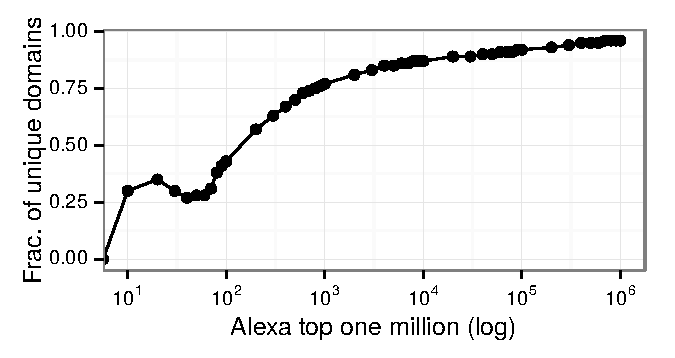
\includegraphics[width=0.7\linewidth]{figures/dns-unique-domains.pdf}
	\caption{The fraction of websites on Alexa top one million that has at least
	one unique domain. The vast majority of sites (96.8\%) have unique domains.}
	\label{fig:unique-domains}
\end{figure}

\begin{table}[t]
	\centering
	\caption{Statistics on the number of DNS requests.}
	\begin{tabular}{l c c c c}
	\toprule
	\textbf{DNS Requests} & \textbf{Median} & \textbf{Mean} & \textbf{Min} & \textbf{Max} \\
	\midrule
	per site & 10 & $12.2\pm11.2$ & 1 & 397 \\
	unique per site & 2 & $2.3\pm1.8$ & 0 & 363 \\
	\bottomrule
	\end{tabular}
	\label{tab:dns-requests}
\end{table}

\begin{table}[t]
	\caption{Raw TTLs are unprocessed while Tor TTLs adhere to Tor's TTL clipping.
	The unique prefix is for the TTL of unique domains while min unique only
	considers the unique domains with the minimum TTL for each website.}
	\centering
	\begin{tabular}{l c c}
	\toprule
	\textbf{TTLs (s)} & \textbf{Median} & \textbf{Mean} \\
	\midrule
	% 2016/04/28 15:52:39 DNS records TTL mean 9780.0, std 42930.5, median 255.0, min 0.0, max 604800.0
	raw & 255 & $9780.0\pm42930.5$ \\ % & 0 & 604800 \\
	% 2016/04/28 15:44:05 DNS records TTL mean 701.5, std 755.3, median 255.0, min 60.0, max 1800.0
	Tor & 255 & $701.5\pm755.3$ \\ %& 60 & 1800 \\
	% 2016/04/28 15:52:39 	unique domain TTL mean 13022.2, std 35054.4, median 900.0, min 0.0, max 604800.0
	unique raw & 900 & $13022.2\pm35054.4$ \\ %& 0 & 604800 \\
	% 2016/04/28 15:44:05 	unique domain TTL mean 1005.3, std 789.6, median 900.0, min 60.0, max 1800.0
	unique Tor & 900 & $1005.3\pm789.6$ \\ %& 60 & 1800 \\
	% 2016/04/28 15:52:39 	unique domain _min_ TTL mean 3833.9, std 11073.6, median 60.0, min 0.0, max 604800.0
	min unique raw & 60 & $3833.9\pm11073.6$ \\ % & 0 & 604800 \\
	% 2016/04/28 15:44:05 	unique domain _min_ TTL mean 644.2, std 763.8, median 60.0, min 60.0, max 1800.0
	min unique Tor & 60 & $644.2\pm763.8$ \\ %& 60 & 1800 \\
	\bottomrule
	\end{tabular}
	\label{tab:ttls}
\end{table}

\fixme{Consider a second round of 5x1M and see if they are stable? Another
option is to cross-validate.}

% TL;DR: unique domains are useful.
Motivated by the above results we construct a na\"{\i}ve website classifier:
map each unique domain in a set of DNS requests to the corresponding website.
Note that it is highly likely that website classification can be made
significantly more accurate if we account for TTLs, order of requests, per-exit
partitioning of DNS requests, and website popularity.

\subsection{Augmenting WF attacks with DNS data}
\fixme{Our approaches are generic for any WF attack (with minor caveats)}
As a baseline we use the Wa-kNN website fingerprinting attack by
Wang et al.~\cite{Wang2014a}. Wa-kNN is a k-nearest neighbour classifier with
a custom weightlearning algorithm (WLLCC~\cite{WangThesis}). From traffic traces
between Tor clients and their guard, Wa-kNN extracts a number of features used
for site classification.
In the training phase, WLLCC adjusts weights of features extracted from sites
of known classes such that the distance between instances of the same site (class) are minimized (collapsed).
In the testing phase, Wa-kNN determines the distance of a testing trace to all
known training traces. The distance calculation produced the $k$ nearest
classes: if all classes are the same, then the testing trace is classified as
that (monitored) class, otherwise it is classified as unmonitored.
For all our classifiers, unless otherwise noted, we set $k=2$. Next, we propose
a number of classifiers that combine Wa-kNN with DNS correlation, followed by
an experimental evaluation.

\subsubsection{Confirmation-based attacks}
We define three classifiers that confirm the output of Wa-kNN with the observed
sites in the DNS data with different goals: high precision (HP), high
 recall (HR), and a merge of HP and HR.

 \begin{description}
 	\item[HP] When Wa-kNN classifies a trace as a monitored site, confirm
	that we observed the same site in the DNS data. If not, overrule Wa-kNN and
	make the final classification unmonitored.
	\item[HR] When Wa-kNN classifies a trace as an unmonitored site, we re-run
	Wa-kNN with $k+1$ and look if there is any class that occured $k$ times.
	If that was the case, and we observed the site (class) in the DNS data,
	then we overrule Wa-kNN and make the final classification the observed class.
	\item[Merge] If the Wa-kNN classifies a trace as a monitored site, take the
	output of HP, otherwise the output from HR.
 \end{description}

The HP classifier increases false negatives but reduces the number of false
positives. The HR classifier reduces confusion with one close neighbour in
Wa-kNN, reducing false negatives but increasing false positives.

\subsubsection{Close-the-world attacks}
Observing DNS requests results in a list of observed sites that are a subset of
the monitored sites.
For our close-the-world classifier we ``close the world''
on a modified Wa-kNN classifier by only considering the distance to observed
sites when calculating the $k$-nearest neighbours. The classifier still
considers the distance to all open instances to capture unmonitored sites.
